\begin{name}
	{Biên soạn: Thầy Bùi Mạnh Tiến và Thầy Lê Nguyễn Viết Tường \& Phản biện: Thầy Lê Nguyễn Viết Tường và Thầy Bùi Mạnh Tiến}
	{Đề thi GHK1 - Nguyễn Trãi - Quảng Nam, năm 2020 - 2021}
\end{name}
	\setcounter{ex}{0}\setcounter{bt}{0}
	\Opensolutionfile{ans}[ans/ans-2-GHK1-33-NguyenTrai-QuangNam-21]
\begin{ex}%[Giữa học kì 1, THPT Nguyễn Trãi Quảng Nam, 2020-2021]%[Bùi Mạnh Tiến, 12EX3]%[2H1Y2-2]
	Tâm của tất cả các mặt một hình lập phương là các đỉnh của hình nào sau đây?
	\choice
	{Lục giác đều}
	{Ngũ giác đều}
	{\True Bát diện đều}
	{Tứ diện đều}
	\loigiai{
		\immini
		{
			Tâm của tất cả các mặt của một hình lập phương là các đỉnh của một bát diện đều.
		}
		{
			\begin{tikzpicture}[line join = round, line cap = round,>=stealth,font=\footnotesize,scale=0.7]
			\def\h{5}
			\def\x{5}
			\path 
			(0,0) coordinate (A)
			(-1.5,-2) coordinate (B)
			($(A)+(\x,0)$) coordinate (D)
			($(B)+(\x,0)$) coordinate (C)
			($(A)+(0,\h)$) coordinate (A')
			($(B)+(0,\h)$) coordinate (B')
			($(C)+(0,\h)$) coordinate (C')
			($(D)+(0,\h)$) coordinate (D')
			($(A')!0.5!(B)$) coordinate (M)
			($(B')!0.5!(C)$) coordinate (N)
			($(C')!0.5!(D)$) coordinate (P)
			($(D')!0.5!(A)$) coordinate (Q)
			($(A')!0.5!(C')$) coordinate (S)
			($(A)!0.5!(C)$) coordinate (R)
			;
			\draw[dashed] (A') -- (A) -- (D) (A) -- (B) (S) -- (M) -- (R) (S) -- (N) -- (R) (S) -- (P) -- (R) (S) -- (Q) -- (R) (M) -- (N) -- (P) -- (Q) -- (M);
			\draw (A') -- (B') -- (C') -- (D') -- cycle
			(B) -- (C) -- (D)
			(A) -- (A') (B) -- (B') (C) -- (C') (D) -- (D')
			;
			\foreach \x/\g in {A/0,B/0,C/0,D/0,A'/0,B'/0,C'/0,D'/0,M/0,N/0,P/0,Q/0,R/0,S/0} \fill[black](\x) circle (1.8pt)+(\g:5mm);
			
			\end{tikzpicture}
		}
	}
\end{ex}

\begin{ex}%[Giữa học kì 1, THPT Nguyễn Trãi Quảng Nam, 2020-2021]%[Bùi Mạnh Tiến, 12EX3]%[2D1Y1-1]
	Cho hàm số $y=\dfrac{2x+5}{x-2}$. Tìm mệnh đề đúng trong các mệnh đề sau
	\choice
	{Hàm số nghịch biến trên $\mathbb{R}\setminus \left\{2\right\}$}
	{Hàm số nghịch biến trên khoảng $(-\infty;3)$}
	{\True Hàm số nghịch biến trên các khoảng $(-\infty;2)$ và $(2;+\infty)$}
	{Hàm số nghịch biến trên $(-\infty;-2)\cup (-2;+\infty)$}
	\loigiai{
		TXĐ: $\mathscr{D}=\mathbb{R}\setminus \left\{2\right\}$.\\
		Ta có $y'=\dfrac{-9}{(x-2)^2}<0$, với $\forall x\in \mathscr{D}$.\\
		Suy ra hàm số nghịch biến trên các khoảng $(-\infty;2)$ và $(2;+\infty)$.
	}
\end{ex}

\begin{ex}%[Giữa học kì 1, THPT Nguyễn Trãi Quảng Nam, 2020-2021]%[Bùi Mạnh Tiến, 12EX3]%[2D1Y2-2]
	Cho hàm số có bảng biến thiên ở hình bên dưới. Khẳng định nào sau đây là khẳng định \textbf{sai}?
	\begin{center}
		
\begin{tikzpicture}[>=stealth,scale=1]
			\tkzTabInit[lgt=1.2,espcl=2.5]
			{$x$ /0.6, $f’(x)$ /0.6, $f(x)$ /2}
			{$-\infty$,$0$,$2$,$+\infty$}
			\tkzTabLine{ ,-,z,+,z,-, }
			\tkzTabVar{+/$+\infty$,-/$1$,+/$3$,-/$-\infty$}
		\end{tikzpicture}
	\end{center}
	\choice
	{Hàm số có $2$ cực trị}
	{\True Giá trị cực tiểu của hàm số bằng $0$}
	{Hàm số đạt cực tiểu tại $x=0$}
	{Hàm số đạt cực đại tại $x=2$}
	\loigiai{
		Từ bảng biến thiên ta thấy hàm số đạt cực tiểu tại điểm $x=0$ và giá trị cực tiểu của hàm số là $y_{CT}=1$.
	}
\end{ex}

\begin{ex}%[Giữa học kì 1, THPT Nguyễn Trãi Quảng Nam, 2020-2021]%[Bùi Mạnh Tiến, 12EX3]%[2D1Y1-2]
	\immini
	{
		Cho hàm số $y=f(x)$ có đồ thị như hình vẽ sau. Hàm số đã cho đồng biến trên khoảng nào dưới đây?
		\choice
		{$(0;1)$}
		{$(-\infty;4)$}
		{\True $(1;+\infty)$}
		{$(-1;1)$}
	}
	{
		\begin{tikzpicture}[line join = round, line cap = round,>=stealth,font=\footnotesize,scale=1]
		\def \xmax{2.5};
		\def \xmin{-2.5};
		\def \ymax{1.5};
		\def \ymin{-3.5};
		\clip (\xmin-0.1,\ymin-0.1) rectangle (\xmax+0.2,\ymax+0.2);
		\draw[->] (\xmin,0) -- (\xmax,0) node[below] {$x$};
		\draw[->] (0,\ymin) -- (0,\ymax) node[left] {$y$};
		\draw (0,0) node[below left] {$O$};
		\draw[samples=100,domain=-1.8:1.8,smooth] plot (\x, {(\x)^4-2*(\x)^2-2});
		\draw[dashed] (-1,0) -- (-1,-3) -- (1,-3) -- (1,0); 
		\fill (-1,0) circle (1pt);
		\fill (1,0) circle (1pt);
		\fill (0,-2) circle (1pt);
		\fill (0,-3) circle (1pt);
		\draw (-1,0) node[above] {$-1$};
		\draw (1,0) node[above] {$1$};
		\draw (0,-2) node[above left] {$-2$};
		\draw (0,-3) node[above left] {$-3$};
		\end{tikzpicture}
	}
	\loigiai{
		Từ đồ thị ta thấy hàm số đồng biến trên các khoảng $(-1;0)$ và $(1;+\infty)$.
	}
\end{ex}

\begin{ex}%[Giữa học kì 1, THPT Nguyễn Trãi Quảng Nam, 2020-2021]%[Bùi Mạnh Tiến, 12EX3]%[2H1Y3-3]
	Cho khối chóp $S.ABC$, trên ba cạnh $SA$, $SB$, $SC$ lần lượt lấy ba điểm $A'$, $B'$, $C'$ sao cho $SA'=\dfrac{1}{6}SA$, $SB'=\dfrac{1}{5}SB$, $SC'=\dfrac{1}{3}SC$. Gọi $V$ và $V'$ lần lượt là thể tích của các khối chóp $S.ABC$ và $S.A'B'C'$, Khi đó tỉ số $\dfrac{V'}{V}$ là
	\choice
	{$14$}
	{\True $\dfrac{1}{90}$}
	{$\dfrac{1}{14}$}
	{$90$}
	\loigiai{
		\immini
		{
			Ta có $\dfrac{V'}{V}=\dfrac{SA'}{SA}\cdot \dfrac{SB'}{SB}\cdot \dfrac{SC'}{SC}=\dfrac{1}{6}\cdot \dfrac{1}{5}\cdot \dfrac{1}{3}=\dfrac{1}{90}$.
		}
		{
			\begin{tikzpicture}[line join = round, line cap = round,>=stealth,font=\footnotesize,scale=0.8]
				\tkzDefPoints{0/0/A,1.5/-2/B,5/0/C,2/4/S}
				\coordinate (A') at ($(S)!1/6!(A)$);
				\coordinate (B') at ($(S)!1/5!(B)$);
				\coordinate (C') at ($(S)!1/3!(C)$);
				\pgfresetboundingbox
				\tkzDrawSegments(S,A S,B S,C A,B B,C A',B' B',C')
				\tkzDrawSegments[dashed](A,C A',C')
				\foreach \x/\g in {A/180,B/-90,C/0,S/90,A'/180,B'/-150,C'/0} \fill[black](\x) circle (1.3pt)+(\g:4mm) node{$\x$};
			\end{tikzpicture}
		}
	}
\end{ex}

\begin{ex}%[Giữa học kì 1, THPT Nguyễn Trãi Quảng Nam, 2020-2021]%[Bùi Mạnh Tiến, 12EX3]%[2D1Y3-1]
	\immini
	{
		Cho hàm số $y=f(x)$ có đồ thị như hình vẽ sau. Gọi $M$ là giá trị lớn nhất của hàm số trên đoạn $[2;3]$. Tìm mệnh đề đúng.
		\choice
		{$M=2$}
		{$M=1$}
		{\True $M=5$}
		{$M=3$}
	}
	{
		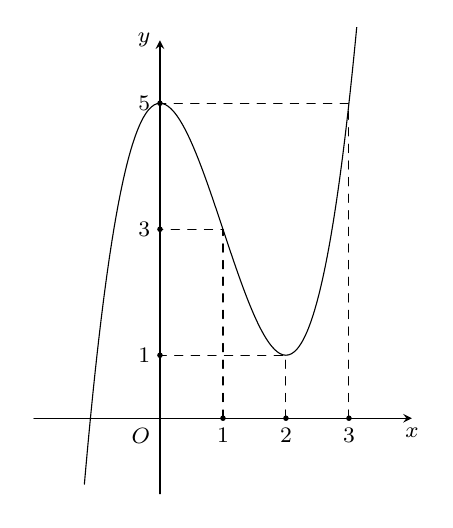
\begin{tikzpicture}[line join = round, line cap = round,>=stealth,font=\footnotesize,scale=0.8]
		\def \xmax{4};
		\def \xmin{-2};
		\def \ymax{6};
		\def \ymin{-1.2};
		\clip (\xmin-0.1,\ymin-0.1) rectangle (\xmax+0.2,\ymax+0.2);
		\draw[->] (\xmin,0) -- (\xmax,0) node[below] {$x$};
		\draw[->] (0,\ymin) -- (0,\ymax) node[left] {$y$};
		\draw (0,0) node[below left] {$O$};
		\draw[samples=100,domain=-1.2:3.2,smooth] plot (\x, {(\x)^3-3*(\x)^2+5});
		\draw[dashed] (1,0) -- (1,3) -- (0,3) (2,0) -- (2,1) -- (0,1) (3,0) -- (3,5) -- (0,5);
		\draw (1,0) node[below] {$1$};
		\draw (2,0) node[below] {$2$};
		\draw (3,0) node[below] {$3$};
		\draw (0,1) node[left] {$1$}; 
		\draw (0,3) node[left] {$3$};
		\draw (0,5) node[left] {$5$};
		\foreach \x in {1,2,3}
		\fill (\x,0) circle (1.25pt);
		\foreach \y in {1,3,5}
		\fill (0,\y) circle (1.25pt);
		\end{tikzpicture}
	}
	\loigiai{
		Từ đồ thị ta thấy $\max\limits_{x \in [2;3]} f(x)=5\Rightarrow M=5$.
	}
\end{ex}

\begin{ex}%[Giữa học kì 1, THPT Nguyễn Trãi Quảng Nam, 2020-2021]%[Bùi Mạnh Tiến, 12EX3]%[2H1Y3-2]
	Tính thể tích của khối lập phương $ABCD.A'B'C'D'$ có $AD=3a$.
	\choice
	{$3a^3$}
	{$9a^3$}
	{\True $27a^3$}
	{$3a^2$}
	\loigiai{
		\immini
		{
			$AD=3a$ là một cạnh của hình lập phương do đó thể tích của hình lập phương là
			\begin{align*}
				V=(3a)^3=27a^3.
			\end{align*}
		}
		{
			\begin{tikzpicture}[line join = round, line cap = round,>=stealth,font=\footnotesize,scale=0.7]
				\def \h{5};
				\tkzDefPoints{0/0/A,5/0/D,-2/-2/B}
				\coordinate (C) at ($(B)+(D)-(A)$);
				\coordinate (A') at ($(A)+(0,\h)$);
				\coordinate (B') at ($(B)+(0,\h)$);
				\coordinate (C') at ($(C)+(0,\h)$);
				\coordinate (D') at ($(D)+(0,\h)$);
				\pgfresetboundingbox
				\tkzDrawSegments(B,C C,D B,B' C,C' D,D' A',B' B',C' C',D' D',A')
				\tkzDrawSegments[dashed](A,A' A,B A,D)
				\foreach \x/\g in {A/180,B/-90,C/-90,D/0,A'/90,B'/180,C'/0,D'/0} \fill[black](\x) circle (1.3pt)+(\g:4mm) node{$\x$};
			\end{tikzpicture}
		}

	}
\end{ex}

\begin{ex}%[Giữa học kì 1, THPT Nguyễn Trãi Quảng Nam, 2020-2021]%[Bùi Mạnh Tiến, 12EX3]%[2H1Y1-1]
	Mỗi đỉnh của một hình đa diện là đỉnh chung của ít nhất mấy mặt?
	\choice
	{năm mặt}
	{hai mặt}
	{bốn mặt}
	{\True ba mặt}
	\loigiai{
		Mỗi đỉnh của một hình đa diện là đỉnh chung của ít nhất ba mặt.
	}
\end{ex}

\begin{ex}%[Giữa học kì 1, THPT Nguyễn Trãi Quảng Nam, 2020-2021]%[Bùi Mạnh Tiến, 12EX3]%[2D1Y5-3]
	Cho hàm số $f(x)$ có bảng biến thiên như hình dưới. Số nghiệm thực của phương trình $f(x)=\dfrac{4}{3}$ là
	\begin{center}
		
\begin{tikzpicture}[>=stealth,scale=1]
			\tkzTabInit[lgt=1.2,espcl=2.5]
			{$x$ /0.6, $f’(x)$ /0.6, $f(x)$ /2}
			{$-\infty$,$1$,$3$,$+\infty$}
			\tkzTabLine{ ,+,z,-,z,+, }
			\tkzTabVar{-/$-\infty$,+/$2$,-/$-2$,+/$+\infty$}
		\end{tikzpicture}
	\end{center}
	\choice
	{$2$}
	{$0$}
	{\True $3$}
	{$4$}
	\loigiai{
		Số nghiệm của phương trình $f(x)=\dfrac{4}{3}$ chính là số giao điểm của hai đồ thị $y=f(x)$ và $y=\dfrac{4}{3}$.
		\begin{center}
			\begin{tikzpicture}[>=stealth,scale=1]
			\tkzTabInit[lgt=1.2,espcl=2.5]
			{$x$ /0.6, $f’(x)$ /0.6, $f(x)$ /2}
			{$-\infty$,$1$,$3$,$+\infty$}
			\tkzTabLine{ ,+,z,-,z,+, }
			\tkzTabVar{-/$-\infty$,+/$2$,-/$-2$,+/$+\infty$}
			\coordinate (A) at ($(N12)!0.45!(N13)$);
			\coordinate (B) at ($(N42)!0.45!(N43)$);
			\draw (A) -- (B) node[below left] {$y=\dfrac{4}{3}$};
			\end{tikzpicture}
		\end{center}
		Từ bảng biến thiên ta thấy đường thẳng $y=\dfrac{4}{3}$ cắt đồ thị hàm số $y=f(x)$ tại $3$ điểm phân biệt, do đó phương trình $f(x)=\dfrac{4}{3}$ có $3$ nghiệm phân biệt.
	}
\end{ex}

\begin{ex}%[Giữa học kì 1, THPT Nguyễn Trãi Quảng Nam, 2020-2021]%[Bùi Mạnh Tiến, 12EX3]%[2D1Y4-1]
	Tiệm cận đứng của đồ thị hàm số $y=\dfrac{2x-2}{x-3}$ là
	\choice
	{\True $x=3$}
	{$x=-3$}
	{$y=2$}
	{$y=3$}
	\loigiai{
		TXĐ: $\mathscr{D}=\mathbb{R}\setminus \{3\}$.\\
		Vì $\lim \limits_{x \to 3^{+}} \dfrac{2x-2}{x-3}=+\infty$ và $\lim \limits_{x \to 3^{-}} \dfrac{2x-2}{x-3}=-\infty$ nên tiệm cận đứng của đồ thị hàm số $y=\dfrac{2x-2}{x-3}$ là $x=3$.
	}
\end{ex}

\begin{ex}%[Giữa học kì 1, THPT Nguyễn Trãi Quảng Nam, 2020-2021]%[Bùi Mạnh Tiến, 12EX3]%[2H1Y3-2]
	Cho khối lăng trụ có diện tích đáy bằng $B$ và chiều cao bằng $h$ . Tính thể tích V của khối lăng trụ đã cho.
	\choice
	{$V=\dfrac{1}{3}Bh$}
	{\True $V=Bh$}
	{$V=3Bh$}
	{$V=\dfrac{1}{2}Bh$}
	\loigiai{
		Thể tích khối lăng trụ có diện tích đáy là $B$, chiều cao $h$ là $V=B\cdot h$.
	}
\end{ex}

\begin{ex}%[Giữa học kì 1, THPT Nguyễn Trãi Quảng Nam, 2020-2021]%[Bùi Mạnh Tiến, 12EX3]%[2H1Y2-2]
	Khối lập phương là khối đa diện đều loại
	\choice
	{\True $\left\{4;3\right\}$}
	{$\left\{3;4\right\}$}
	{$\left\{3;5\right\}$}
	{$\left\{5;3\right\}$}
	\loigiai{
		Khối lập phương là khối đa diện đều loại $\{4;3\}$.
	}
\end{ex}


\begin{ex}%[Giữa học kì 1, THPT Nguyễn Trãi Quảng Nam, 2020-2021]%[Lê Nguyễn Viết Tường, 12EX3-2021]%[2H1Y3-2]
	Hình chóp $S.ABC$ có diện tích đáy bằng $2019$ dm$^2$, đường cao $SA=2020$ dm. Tính thể tích $V$ của khối chóp $S.ABC$.
	\choice
	{$V=4078350$ dm$^3$}
	{$V=1359460$ dm}
	{\True $V=1359460$ dm$^3$}
	{$V=4078350$ dm}
	\loigiai{
		Ta có $V=\dfrac{1}{3}\cdot 2019\cdot 2020=1359460$ dm$^3$.
	}
\end{ex}

\begin{ex}%[Giữa học kì 1, THPT Nguyễn Trãi Quảng Nam, 2020-2021]%[Lê Nguyễn Viết Tường, 12EX3-2021]%[2H1Y3-2]
	Cho hình chóp $S.ABC$ có $SA$ vuông góc với mặt phẳng $(ABC)$, $\triangle ABC$ là tam giác vuông tại $B$. Tính thể tích khối chóp $S.ABC$, biết $AB=a$, $AC=2a$, $SA=3a$.
	\choice
	{$2a^3$}
	{$6a^3$}
	{$\dfrac{3\sqrt{3}a^3}{2}$}
	{\True $\dfrac{a^3\sqrt{3}}{2}$}
	\loigiai{
		\immini{
			$\triangle ABC$ vuông tại $B \Rightarrow BC=\sqrt{AC^2-AB^2}=a\sqrt{3}$.\\
			Khi đó $S_{\triangle ABC}=\dfrac{1}{2}AB\cdot BC=\dfrac{a^2\sqrt{3}}{2}$.\\
			Thể tích của khối chóp $S.ABC$ là $$V=\dfrac{1}{3}\cdot SA\cdot S_{\triangle ABC}=\dfrac{1}{3}\cdot 3a\cdot \dfrac{a^2\sqrt{3}}{2}=\dfrac{a^3\sqrt{3}}{2}.$$
		}{
			\begin{tikzpicture}[scale=.6, font=\footnotesize, line join=round, line cap=round, >=stealth]
			\tkzDefPoints{0/0/A,0/5.7/S,5/0/C,2.4/-2/B}
			\tkzDrawSegments[dashed](A,C)
			\tkzDrawSegments[](S,A A,B B,C S,C S,B)
			\tkzLabelPoints[above](S)
			\tkzLabelPoints[left](A)
			\tkzLabelPoints[right](C)
			\tkzLabelPoints[below](B)
			\tkzDrawPoints[fill=black](S,A,B,C)
			\tkzMarkRightAngles(A,B,C)
			\end{tikzpicture}
		}
	}
\end{ex}

\begin{ex}%[Giữa học kì 1, THPT Nguyễn Trãi Quảng Nam, 2020-2021]%[Lê Nguyễn Viết Tường, 12EX3-2021]%[2D1Y1-2]
	Cho hàm số $y=f(x)$ có bảng biến thiên như sau
	\begin{center}
		
\begin{tikzpicture}
		\tkzTabInit
		[nocadre=false,lgt=1.2,espcl=2.5,deltacl=0.6]
		{$x$/0.6, $f'(x)$/0.6, $f(x)$/2}
		{$-\infty$,$-1$,$3$, $+\infty$}
		\tkzTabLine{, +,z,-,z,+, }
		\tkzTabVar{ -/ $-\infty$,+/ $4$,-/ $-2$,+/$+\infty$ }
		\end{tikzpicture}
	\end{center}
	Hàm số đã cho nghịch biến trên khoảng nào dưới đây?
	\choice
	{$(-2;4)$}
	{$(-\infty ;4)$}
	{$(-2;+\infty )$}
	{\True $(-1;3)$}
	\loigiai{
		Dựa vào bảng biến thiên ta có hàm số nghịch biến trên khoảng $(-1;3)$.
	}
\end{ex}

\begin{ex}%[Giữa học kì 1, THPT Nguyễn Trãi Quảng Nam, 2020-2021]%[Bùi Mạnh Tiến, 12EX3]%[2D1B4-1]
	\immini
	{
		Cho hàm số $y=f(x)$ có bảng biến thiên như hình bên. Tìm mệnh đề \textbf{đúng}
		\choice
		{Đồ thị hàm số không có tiệm cận}
		{Đồ thị hàm số có hai tiệm cận ngang}
		{\True Đồ thị hàm số có một tiệm cận ngang}
		{Hàm số xác định trên $\mathbb{R}$}
	}
	{
		
\begin{tikzpicture}[>=stealth,scale=1]
		\tkzTabInit[lgt=1.2,espcl=2.5]
		{$x$/0.6,$f’(x)$/0.6,$f(x)$/2}
		{$-\infty$,$-1$,$+\infty$}
		\tkzTabLine{ ,-,d,-,}
		\tkzTabVar{+/$2$,-D+/$-\infty$/$+\infty$,-/$2$}
		\end{tikzpicture}
	}
	\loigiai{
		Từ bảng biến thiên ta thấy
		\begin{itemize}
			\item TXĐ $\mathscr{D}=\mathbb{R}\setminus \{-1\}$.
			\item $\lim \limits_{x \to \pm \infty} f(x)=2\Rightarrow y=2$ là tiệm cận ngang của đồ thị hàm số.
		\end{itemize}
	}
\end{ex}


\begin{ex}%[Giữa học kì 1, THPT Nguyễn Trãi Quảng Nam, 2020-2021]%[Bùi Mạnh Tiến, 12EX3]%[2D1B2-1]
	Hàm số $y=f(x)$ có đạo hàm là $f'(x)=x^2(x-1)^3(3-x)$. Khi đó số điểm cực trị của hàm số là
	\choice
	{$0$}
	{$3$}
	{$1$}
	{\True $2$}
	\loigiai{
		Ta có $f'(x)=0\Leftrightarrow \hoac{& x=0 \\ & x=1\\& x=3.}$\\
		Suy ra bảng xét dấu của $f'(x)$ như sau
		\begin{center}
			
\begin{tikzpicture}[>=stealth,scale=1]
			\tkzTabInit[lgt=1.2,espcl=2.5]
			{$x$ /0.6, $f’(x)$ /0.6}
			{$-\infty$,$0$,$1$,$3$,$+\infty$}
			\tkzTabLine{ ,-,z,-,z,+,z,-, }
			\end{tikzpicture}
		\end{center}
		Ta thấy $f'(x)$ đổi dấu qua $x=1$ và $x=3$ nên hàm số có $2$ điểm cực trị là $x=1$ và $x=3$.
	}
\end{ex}

\begin{ex}%[Giữa học kì 1, THPT Nguyễn Trãi Quảng Nam, 2020-2021]%[Bùi Mạnh Tiến, 12EX3]%[2D1B2-1]
	Hàm số $y=ax^4+bx^2+c$ ($a\ne 0$) có $1$ cực tiểu và $2$ cực đại khi và chỉ khi
	\choice
	{$\heva{& a<0 \\ & b\ge 0}$}
	{$\heva{& a>0 \\ & b\ne 0}$}
	{$\heva{& a>0 \\ & b>0}$}
	{\True $\heva{& a<0 \\ & b>0}$}
	\loigiai{
		\immini
		{
			Hàm trùng phương có $1$ cực tiểu và $2$ cực đại có dáng đồ thị như hình vẽ bên.
			\begin{itemize}
				\item Đồ thị hướng xuống nên $a<0$.
				\item Hàm số có $3$ điểm cực trị nên $a\cdot b<0\Rightarrow b>0$.
			\end{itemize}	
		}
		{
			\begin{tikzpicture}[line join = round, line cap = round,>=stealth,font=\footnotesize,scale=1]
			\def \xmax{2.5};
			\def \xmin{-2.5};
			\def \ymax{1.5};
			\def \ymin{-2};
			\clip (\xmin-0.1,\ymin-0.1) rectangle (\xmax+0.2,\ymax+0.2);
			\draw[->] (0,\ymin) -- (0,\ymax) node[left] {$y$};
			\draw[samples=100,domain=-1.65:1.65,smooth] plot (\x, {-(\x)^4+2*(\x)^2});
			\end{tikzpicture}
		}
	}
\end{ex}

\begin{ex}%[Giữa học kì 1, THPT Nguyễn Trãi Quảng Nam, 2020-2021]%[Lê Nguyễn Viết Tường, 12EX3-2021]%[2D1B2-2]
	Cho hàm số $y=x^4-2x^2+3$. Tìm mệnh đề \textbf{sai} trong các mệnh đề sau
	\choice
	{Hàm số có giá trị cực đại bằng 3}
	{Hàm số có giá trị nhỏ nhất bằng 2}
	{\True Hàm số có giá trị lớn nhất bằng 3}
	{Hàm số có ba điểm cực trị}
	\loigiai{
		Tập xác định: $\mathscr D=\mathbb{R}$.\\
		Ta có $y'=4x^3-4x$; $y'=0\Leftrightarrow \hoac{&x=0\\&x=\pm 1.}$\\
		Với $x=0\Rightarrow y=3$; $x=\pm 1\Rightarrow y=2$.\\
		Bảng biến thiên
		\begin{center}
			
\begin{tikzpicture}
			\tkzTabInit
			[nocadre=false,lgt=1.2,espcl=2.5,deltacl=0.6]
			{$x$/0.6, $f'(x)$/0.6, $f(x)$/2}
			{$-\infty$,$-1$,0,1, $+\infty$}
			\tkzTabLine{, -,z,+,z,-,z,+, }
			\tkzTabVar{ +/$+\infty$,-/ $2$,+/ $3$,-/$2$,+/$+\infty$ }
			\end{tikzpicture}
		\end{center}
		Hàm số đã cho không có giá trị lớn nhất trên $\mathbb{R}$.
	}
\end{ex}

\begin{ex}%[Giữa học kì 1, THPT Nguyễn Trãi Quảng Nam, 2020-2021]%[Lê Nguyễn Viết Tường, 12EX3-2021]%[2D1B5-4]
	Số giao điểm của hai đồ thị hàm số $y=x^4-2x^2+2$ và $y=-x^2+4$ là
	\choice
	{\True $2$}
	{$0$}
	{$1$}
	{$4$}
	\loigiai{
		Xét phương trình hoành độ giao điểm ta có $$x^4-2x^2+2=-x^2+4\Leftrightarrow x^4-x^2-2=0\Leftrightarrow\hoac{&x^2=-1\\&x^2=2}\Leftrightarrow\hoac{&x=\sqrt{2}\\&x=-\sqrt{2}.}$$
		Vậy số giao điểm của hai đồ thị hàm số là $2$.
	}
\end{ex}

\begin{ex}%[Giữa học kì 1, THPT Nguyễn Trãi Quảng Nam, 2020-2021]%[Lê Nguyễn Viết Tường, 12EX3-2021]%[2D1B5-1]
	\immini{
		Đường cong trong hình vẽ bên là đồ thị của hàm số nào?
		\choice
		{$y=x^4+2x^2+1$}
		{$y=x^4+1$}
		{\True$y=-x^4+2x^2+1$}
		{$y=-x^4-2x^2+1$}
	}{
		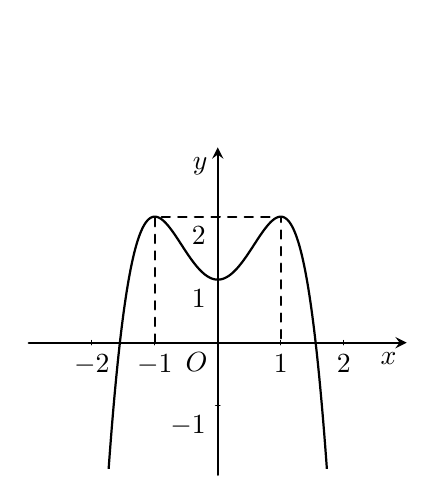
\begin{tikzpicture}[line join=round, line cap=round,>=stealth,thick,scale=.8]
		\tikzset{label style/.style={font=\footnotesize}}
		\tkzInit[xmin=-3.1,xmax=3.1,ymin=-2.2,ymax=3.2]
		\tkzClip
		\draw[->] (-3,0)--(3,0) node[below left] {$x$};
		\draw[->] (0,-2.1)--(0,3.1) node[below left] {$y$};
		\draw (0,0) node [below left] {$O$};
		\foreach \x in {-2,-1,1,2}
		\draw[thin] (\x,1pt)--(\x,-1pt) node [below] {$\x$};
		\foreach \y in {-1,1,2}
		\draw[thin] (1pt,\y)--(-1pt,\y) node [below left] {$\y$};
		\begin{scope}
		\clip (-2.5,-2) rectangle (2.5,5);
		\draw[samples=200,domain=-2:2,smooth,variable=\x] plot (\x,{-(\x)^4+2*(\x)^2+1});
		\draw[dashed] (-1,0)--(-1,2)--(1,2)--(1,0);
		\end{scope}
		\end{tikzpicture}
	}
	\loigiai{
		Đồ thị của đường cong trong hình vẽ là đồ thị của hàm số dạng $y=ax^4+bx^2+c$.\\
		Dựa vào hình dáng đồ thị ta suy ra $a<0$.\\
		Thế $x=1$ vào $y=-x^4+2x^2+1$ ta được $y=2$.\\
		Vậy đường cong trong hình vẽ bên là đồ thị của hàm số $y=-x^4+2x^2+1$.
	}
\end{ex}

\begin{ex}%[Giữa học kì 1, THPT Nguyễn Trãi Quảng Nam, 2020-2021]%[Lê Nguyễn Viết Tường, 12EX3-2021]%[2D1B5-1]
	\immini{
		Đồ thị của hàm số nào dưới đây có dạng như đường cong trong hình vẽ bên?
		\choice
		{$y=x^4-2x^3+3$}
		{\True$y=x^3-3x-1$}
		{$y=-x^3+3x^2+3$}
		{$y=-x^4+2x^3+3$}
	}{
		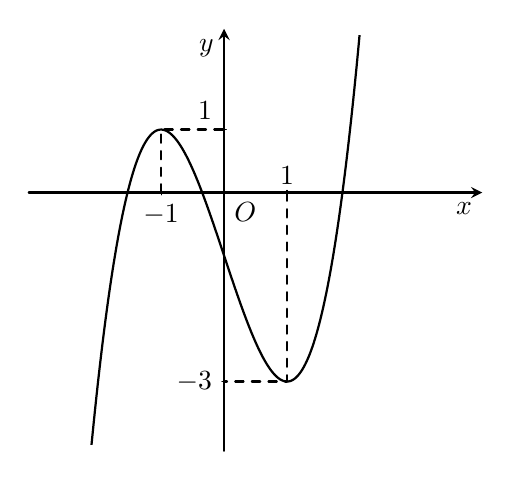
\begin{tikzpicture}[line join=round, line cap=round,>=stealth,thick,scale=.8]
		\tikzset{label style/.style={font=\footnotesize}}
		\draw[->] (-3.1,0)--(4.1,0) node[below left] {$x$};
		\draw[->] (0,-4.1)--(0,2.6) node[below left] {$y$};
		\draw (0,0) node [below right] {$O$};
		\foreach \x in {-1}
		\draw[thin] (\x,1pt)--(\x,-1pt) node [below] {$\x$};
		\draw[thin] (1,1pt)--(1,-1pt) node [above]{1};
		\foreach \y in {1}
		\draw[thin] (1pt,\y)--(-1pt,\y) node [above left] {$\y$};
		\draw[thin] (1pt,-3)--(-1pt,-3) node [left] {$-3$};
		\begin{scope}
		\clip (-3,-4) rectangle (4,2.5);
		\draw[samples=200,domain=-2.5:2.5,smooth,variable=\x] plot (\x,{(\x)^3-3*(\x)-1});
		\draw[dashed] (-1,0)--(-1,1)--(0,1);
		\draw[dashed] (1,0)--(1,-3)--(0,-3);
		\end{scope}
		\end{tikzpicture}
	}
	\loigiai{
		Đường cong ở hình bên là đồ thị của hàm số dạng $y=ax^3+bx^2+cx+d$.\\
		Dựa vào hình dáng đồ thị ta có $a>0$.\\
		Vậy đường cong trong hình vẽ là đồ thị của hàm số $y=x^3-3x-1$.
	}
\end{ex}

\begin{ex}%[Giữa học kì 1, THPT Nguyễn Trãi Quảng Nam, 2020-2021]%[Lê Nguyễn Viết Tường, 12EX3-2021]%[2D1B3-1]
	Giá trị nhỏ nhất của hàm số $y=f(x)=x^3-2x^2$ trên đoạn $[-1;3]$ là
	\choice
	{$0$}
	{$9$}
	{$-\dfrac{32}{27}$}
	{\True $-3$}
	\loigiai{
		Xét trên đoạn $[-1;3]$, ta có\\
		$f'(x)=3x^2-4x$; $f'(x)=0\Leftrightarrow \hoac{&x=0\\&x=\dfrac{4}{3}.}$\\
		Hàm số đã cho liên tục trên đoạn $[-1;3]$, đồng thời \\
		$f(-1)=-3$;\quad$f(0)=0$;\quad$f\left (\dfrac{4}{3} \right )=-\dfrac{32}{27}$;\quad$f(3)=9$.\\
		Vậy giá trị nhỏ nhất của hàm số trên đoạn $[-1;3]$ là $-3$.
	}
\end{ex}


\begin{ex}%[Giữa học kì 1, THPT Nguyễn Trãi Quảng Nam, 2020-2021]%[Lê Nguyễn Viết Tường, 12EX3-2021]%[2D1B5-4]
	\immini{
		Cho hàm số $y=f(x)$ liên tục trên $\mathbb{R}$ và có đồ thị như hình vẽ bên. Hỏi phương trình $2|f(x)|-1=0$ có bao nhiêu nghiệm dương?
		\choice
		{$2$}
		{$1$}
		{\True $4$}
		{$3$}
	}{
		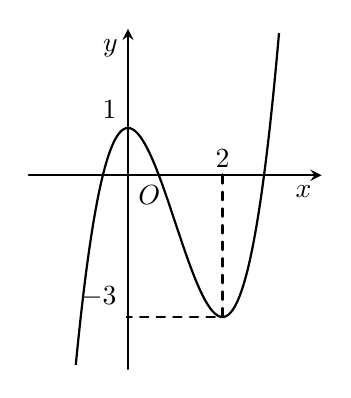
\begin{tikzpicture}[line join=round, line cap=round,>=stealth,thick,scale=.6]
		\tikzset{label style/.style={font=\footnotesize}}
		\draw[->] (-2.1,0)--(4.1,0) node[below left] {$x$};
		\draw[->] (0,-4.1)--(0,3.1) node[below left] {$y$};
		\draw (0,0) node [below right] {$O$};
		\foreach \x in {2}
		\draw[thin] (\x,1pt)--(\x,-1pt) node [above] {$\x$};
		\foreach \y in {-3,1}
		\draw[thin] (1pt,\y)--(-1pt,\y) node [above left] {$\y$};
		\begin{scope}
		\clip (-2,-4) rectangle (3.3,3);
		\draw[samples=200,domain=-2:3.3,smooth,variable=\x] plot (\x,{(\x)^3-3*(\x)^2+1});
		\draw[dashed] (2,0)--(2,-3)--(0,-3);
		\end{scope}
		
		\end{tikzpicture}
	}
	\loigiai{
		\immini
		{
			Xét đồ thị của hàm số $y=\left |f(x) \right |$.
			Số nghiệm của phương trình $2\left |f(x) \right |-1=0$ là số giao điểm của đồ thị hàm số $y=\left |f(x) \right |$ và đường thẳng $y=\dfrac{1}{2}$.\\
			Dựa vào đồ thị phương trình đã cho có $4$ nghiệm dương.
		}
		{
			\begin{tikzpicture}[line join=round, line cap=round,>=stealth,thick,scale=.8]
			\tikzset{label style/.style={font=\footnotesize}}
			\draw[->] (-2.1,0)--(4.1,0) node[below left] {$x$};
			\draw[->] (0,-1.1)--(0,5.1) node[below left] {$y$};
			\draw (-0.1,0) node [below left] {$O$};
			\foreach \y in {1}
			\draw[thin] (1pt,\y)--(-1pt,\y) node [above left] {$\y$};
			\begin{scope}
			\clip (-2,-1) rectangle (3.3,5);
			\draw[samples=200,domain=-2:3.3,smooth,variable=\x] plot (\x,{abs((\x)^3-3*(\x)^2+1)});
			\end{scope}
			\draw (-2.1,0.5)--(4.1,0.5)node[above]{$y=\dfrac{1}{2}$};
			\end{tikzpicture}
		}
	}
\end{ex}


\begin{ex}%[Giữa học kì 1, THPT Nguyễn Trãi Quảng Nam, 2020-2021]%[Lê Nguyễn Viết Tường, 12EX3-2021]%[2D1B2-3]
	Tìm $m$ để hàm số $y=f(x)=\dfrac{1}{3}x^3-mx^2+\left (m^2-m+1 \right )x+1$ đạt cực đại tại điểm $x=1$.
	\choice
	{\True $m=2$}
	{$m=1$}
	{$\hoac{&m=1\\&m=2}$}
	{$m=-2$}
	\loigiai{
		Giả sử $x=1$ là điểm cực đại của hàm số, khi đó ta có 
		\begin{eqnarray*}
			\heva{&f'(1)=0\\&f''(1)<0}&\Leftrightarrow &\heva{&1^2-2m\cdot 1+m^2-m+1=0\\&2\cdot 1-2m<0}\\&\Leftrightarrow &\heva{&\hoac{&m=1\\&m=2}\\&m>1}\\&\Leftrightarrow &m=2.
		\end{eqnarray*}
		Với $m=2$ ta có hàm số $y=f(x)=\dfrac{1}{3}x^3-2x^2+3x+1$.\\
		$f'(x)=x^2-4x+3$; $f'(x)=0\Leftrightarrow x^2-4x+3=0\Leftrightarrow\hoac{&x=1\\&x=3.}$\\
		Bảng biến thiên 
		\begin{center}
			
\begin{tikzpicture}
			\tkzTabInit
			[nocadre=false,lgt=1.2,espcl=2.5,deltacl=0.6]
			{$x$/0.6, $f'(x)$/0.6, $f(x)$/2}
			{$-\infty$,1,3, $+\infty$}
			\tkzTabLine{, +,z,-,z,+, }
			\tkzTabVar{ -/$-\infty$,+/$f(1)$,-/$f(3)$,+/$+\infty$ }
			\end{tikzpicture}
		\end{center}
		Do đó $x=1$ là điểm cực đại của hàm số.\\
		Vậy $m=2$ là giá trị cần tìm.
	}
\end{ex}

\begin{ex}%[Giữa học kì 1, THPT Nguyễn Trãi Quảng Nam, 2020-2021]%[Lê Nguyễn Viết Tường, 12EX3-2021]%[2D1K1-3]
	Có tất cả bao nhiêu giá trị nguyên của tham số $m$ để hàm số $y=\dfrac{mx+8}{2x+m}$ nghịch biến trên khoảng $(0;3)$?
	\choice
	{$9$}
	{$4$}
	{\True $5$}
	{$3$}
	\loigiai{
		Tập xác định: $\mathscr D=\mathbb{R}\setminus\left \{-\dfrac{m}{2} \right \}$.\\
		Hàm số nghịch biến trên khoảng $(0;3)$ $$\Leftrightarrow\heva{&y'\le 0\,\forall x\in (0;3)\\&(0;3)\subset \mathscr D}\Leftrightarrow\heva{&m^2-16\le 0\\&\hoac{&-\dfrac{m}{2}\ge 3\\&-\dfrac{m}{2}\le 0}}\Leftrightarrow\heva{&-4\le m\le 4\\&\hoac{&m\le -6\\&m\ge 0}}\Leftrightarrow 0\le m\le 4.$$
		Mà $m\in\mathbb{Z}$ nên $m\in\left \{0;1;2;3;4 \right \}$.\\
		Vậy có 5 giá trị nguyên của $m$ thỏa yêu cầu bài toán.
	}
\end{ex}

\begin{ex}%[Giữa học kì 1, THPT Nguyễn Trãi Quảng Nam, 2020-2021]%[Lê Nguyễn Viết Tường, 12EX3-2021]%[2D1K2-6]
	Có bao nhiêu giá trị nguyên của tham số $m$ để hàm số $y=\left |x^3-3x^2+m \right |$ có $5$ điểm cực trị?
	\choice
	{$5$}
	{$6$}
	{\True $3$}
	{$4$}
	\loigiai{
		Xét hàm số $f(x)=x^3-3x^2+m$.\\
		Tập xác định: $\mathscr D=\mathbb{R}$.
		Ta có $f'(x)=3x^2-6x\Rightarrow f'(x)=0\Leftrightarrow \hoac{&x=0\\&x=2.}$\\
		Bảng biến thiên
		\begin{center}
			
\begin{tikzpicture}
			\tkzTabInit
			[nocadre=false,lgt=1.2,espcl=2.5,deltacl=0.6]
			{$x$/0.6, $f'(x)$/0.6, $f(x)$/2}
			{$-\infty$,$0$,$2$, $+\infty$}
			\tkzTabLine{, +,z,-,z,+, }
			\tkzTabVar{ -/$-\infty$,+/$m$,-/$m-4$,+/$+\infty$ }
			\end{tikzpicture}
		\end{center}
		Dựa vào bảng biến thiên, hàm số $y=\left |f(x) \right |$ có 5 điểm cực trị 
		\begin{align*}
			&\Leftrightarrow y=f(x) \text{ có hai cực trị nằm về hai phía so với trục hoành}\\ 
			&\Leftrightarrow \heva{&m>0\\&m-4<0}\Leftrightarrow 0<m<4.
		\end{align*}
		Khi đó hàm số có 3 điểm cực trị là 3 giao điểm của $y=0$ và $y=|f(x)|$, 1 cực trị có tọa độ $(0;m)$, 1 cực trị có tọa độ $(2;-m+4)$.\\
		Mà $m\in\mathbb{Z}$ nên $m\in\left \{1;2;3 \right \}$.
	}
\end{ex}

\begin{ex}%[Giữa học kì 1, THPT Nguyễn Trãi Quảng Nam, 2020-2021]%[Lê Nguyễn Viết Tường, 12EX3-2021]%[2H1K3-2]
	Lăng trụ $ABC.A'B'C'$ có đáy là tam giác đều cạnh $a$. Hình chiếu vuông góc của $A'$ lên $(ABC)$ trùng với trọng tâm $O$ của tam giác $ABC$. Mặt phẳng $(P)$ chứa $BC$ vuông góc với $AA'$ cắt lăng trụ theo thiết diện có diện tích bằng $\dfrac{a^2\sqrt{3}}{8}$. Thể tích khối đa diện $AC'BA'$ là
	\choice
	{\True $\dfrac{a^3\sqrt{3}}{18}$}
	{$\dfrac{a^3\sqrt{3}}{36}$}
	{$\dfrac{a^3\sqrt{3}}{12}$}
	{$\dfrac{a^3\sqrt{3}}{6}$}
	\loigiai{
		\immini
		{
			Gọi $M$ là trung điểm của $BC$.\\
			Ta có $\heva{&BC\perp AM\\&BC\perp A'O}\Rightarrow BC\perp (AA'M)\Rightarrow BC\perp AA'$.\\
			Kẻ $MH\perp AA'$ tại $H$.\\
			Ta có $\heva{&AA'\perp MH\\&AA'\perp BC}\Rightarrow AA'\perp (BCH)\Rightarrow (P)\equiv (BCH)$.\\
			$S_{\triangle BCH}=\dfrac{1}{2}BC\cdot HM\Rightarrow HM=\dfrac{a\sqrt{3}}{4}$.
		}
		{
			\begin{tikzpicture}[scale=.7, font=\footnotesize, line join=round, line cap=round, >=stealth]
			\tkzDefPoints{0/0/A,5/0/C,2.2/-2/B}
			\tkzDefMidPoint(B,C)\tkzGetPoint{M}
			\tkzDefBarycentricPoint(A=1,M=2)\tkzGetPoint{O}
			\coordinate (A') at ($(O)+(0,6)$);
			\tkzDefPointBy[translation=from A to C](A')\tkzGetPoint{C'}
			\tkzDefPointBy[translation=from A to B](A')\tkzGetPoint{B'}
			\tkzDefBarycentricPoint(A=2.5,A'=1.5)\tkzGetPoint{H}
			\tkzDrawSegments[dashed](A',O A,C A,M M,H C,H M,H)
			\tkzDrawSegments[](A',B' B',C' C',A' A,B B,C A,A' B,B' C,C' B,H)
			\tkzDrawPoints[fill=black](A,B,C,A',B',C',H,O,M)
			\tkzLabelPoints[above](A',B',C')
			\tkzLabelPoints[left](H,A)
			\tkzLabelPoints[below](B,O)
			\tkzLabelPoints[right](M,C)
			\end{tikzpicture}
		}
		\noindent
		$\triangle AHM$ vuông tại $H\Rightarrow AH=\sqrt{AM^2-HM^2}=\sqrt{\left (\dfrac{a\sqrt{3}}{2} \right )^2-\left (\dfrac{a\sqrt{3}}{4} \right )^2}=\dfrac{3a}{4}$.\\
		$\triangle A'AO\backsim\triangle MAH\Rightarrow \dfrac{A'O}{AO}=\dfrac{HM}{AH}\Rightarrow A'O=\dfrac{AO\cdot HM}{AH}=\dfrac{a}{3}$.\\
		Thể tích khối trụ là $V_1=A'O\cdot S_{\triangle ABC}=\dfrac{a}{3}\cdot\dfrac{a^2\sqrt{3}}{4}=\dfrac{a^3\sqrt{3}}{12}$.\\
		Thể tích khối đa diện $C'ABC$ là $V_2=\dfrac{1}{3}\cdot A'O\cdot S_{\triangle ABC}=\dfrac{a^3\sqrt{3}}{36}$.\\
		Thể tích khối đa diện $AC'BA'$ là $V=V_1-V_2=\dfrac{a^3\sqrt{3}}{18}$.
	}
\end{ex}

\begin{ex}%[Giữa học kì 1, THPT Nguyễn Trãi Quảng Nam, 2020-2021]%[Lê Nguyễn Viết Tường, 12EX3-2021]%[2D1K1-3]
	\immini{
		Cho hàm số $y=f(x)$. Biết hàm số $y=f'(x)$ có đồ thị như hình vẽ bên. Hỏi hàm số $y=f(2-2x)$ nghịch biến trên khoảng nào dưới đây?
		\choice
		{$(2;+\infty )$}
		{$(-\infty ;-1)$ và $(1;+\infty )$}
		{$(-1;+\infty )$}
		{\True $(-\infty ;2)$}
	}{
		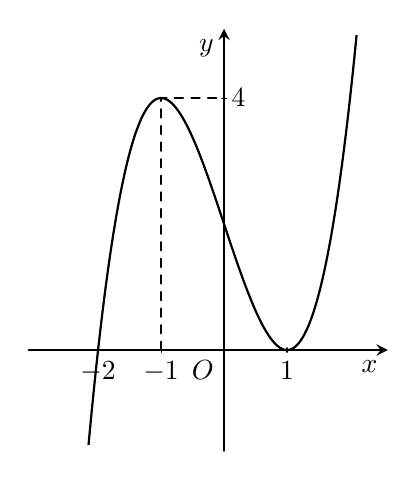
\begin{tikzpicture}[line join=round, line cap=round,>=stealth,thick,scale=.8]
		\tikzset{label style/.style={font=\footnotesize}}
		\draw[->] (-3.1,0)--(2.6,0) node[below left] {$x$};
		\draw[->] (0,-1.6)--(0,5.1) node[below left] {$y$};
		\draw (0,0) node [below left] {$O$};
		\foreach \x in {-2,-1,1}
		\draw[thin] (\x,1pt)--(\x,-1pt) node [below] {$\x$};
		\foreach \y in {4}
		\draw[thin] (1pt,\y)--(-1pt,\y) node [right] {$\y$};
		\begin{scope}
		\clip (-3,-1.5) rectangle (2.5,5);
		\draw[samples=200,domain=-2.3:2.3,smooth,variable=\x] plot (\x,{(\x)^3-3*(\x)+2});
		\draw[dashed] (-1,0)--(-1,4)--(0,4);
		\end{scope}
		
		\end{tikzpicture}
	}
	\loigiai{
		Xét hàm số $g(x)=f(2-2x)\Rightarrow g'(x)=-2f'(2-2x)$.
		$$g'(x)\le 0\Leftrightarrow f'(2-2x)\ge 0\Leftrightarrow 2-2x\ge -2\Leftrightarrow x\le 2.$$
		Vậy hàm số $y=f(2-2x)$ nghịch biến trên khoảng $(-\infty;2 )$.
	}
\end{ex}

\begin{ex}%[Giữa học kì 1, THPT Nguyễn Trãi Quảng Nam, 2020-2021]%[Lê Nguyễn Viết Tường, 12EX3-2021]%[1H3G5-3]
	Cho hình chóp $S.ABCD$ có đáy $ABCD$ là hình bình hành, $AD=a$, $AC=a\sqrt{3}$, $CD=2a$. Tam giác $SCD$ cân tại $S$, tam giác $SBC$ vuông tại $C$. Khoảng cách từ $B$ đến mặt phẳng $SCD$ bằng $\dfrac{a\sqrt{3}}{3}$. Chiều cao $SH$ của hình chóp là
	\choice
	{$\dfrac{a\sqrt{5}}{3}$}
	{\True $\dfrac{2a\sqrt{15}}{15}$}
	{$\dfrac{a\sqrt{15}}{3}$}
	{$\dfrac{a\sqrt{15}}{5}$}
	\loigiai{
		\immini
		{
			Tam giác $ACD$ có $CD^2=AC^2+AD^2$.\\
			Do đó $\triangle ACD$ vuông tại $A$.\\
			Mà $ABCD$ là hình bình hành nên $\widehat{CAD}=\widehat{ACB}=90^\circ$ hay $BC\perp AC$.\\
			Lại có $BC\perp SC$ nên $BC\perp (SAC)$.\\
			Kẻ $SH\perp AC$ tại $H$, ta có
			Từ $\heva{&SH\perp AC\\&SH\perp BC\text{ (do }BC\perp (SAC),SH\subset (SAC))}$\\
			$\Rightarrow SH\perp (ABCD)$.
		}
		{
			\begin{tikzpicture}[scale=.7, font=\footnotesize, line join=round, line cap=round, >=stealth]
			\tkzDefPoints{0/0/A,-2/-2/B,5.5/0/D,3.5/-2/C}
			\tkzDefBarycentricPoint(A=3,C=1)\tkzGetPoint{H}
			\coordinate (S) at ($(H)+(0,5.5)$);
			\tkzDefMidPoint(C,D)\tkzGetPoint{I}
			\tkzDefBarycentricPoint(S=2,I=3)\tkzGetPoint{K}
			\tkzDrawSegments[dashed](S,H S,A A,B A,C A,D H,I H,K)
			\tkzDrawSegments[](S,B S,C S,D B,C C,D S,I)
			\tkzLabelPoints[above](S)
			\tkzLabelPoints[left](A)
			\tkzLabelPoints[below left](B,H)
			\tkzLabelPoints[below right](C)
			\tkzLabelPoints[right](D,I,K)
			\tkzDrawPoints[fill=black](S,A,B,C,D,H)
			\end{tikzpicture}
		}
		\noindent
		Ta có $\sin C=\dfrac{AD}{CD}=\dfrac{\sqrt{3}}{2}\Rightarrow\widehat{ACD}=30^\circ$.\\
		Gọi $I$ là trung điểm của $CD\\ \Rightarrow SI\perp CD$ (do $\triangle SCD$ cân tại $S$) $\Rightarrow HI\perp CD$ (định lý 3 đường vuông góc).\\
		Khi đó ta có $HC=IC\cdot\tan\widehat{ACD}=a\cdot\tan 30^\circ =\dfrac{a\sqrt{3}}{3}\Rightarrow HC=\dfrac{2}{3}AC$.\\
		Ta có $\mathrm{d}(B,(SCD))=\mathrm{d}(A,(SCD))=\dfrac{AC}{HC}\cdot\mathrm{d}(H,(SCD))\\ \Rightarrow\mathrm{d}(H,(SCD))=\dfrac{2}{3}\mathrm{d}(B,(SCD))=\dfrac{2a\sqrt{3}}{9}$.\\
		Ta có $\heva{&CD\perp HI\\&CD\perp SH}\Rightarrow CD\perp (SHI)$.\\
		Kẻ $HK\perp SI$ tại $K$, ta có
		$$\heva{&HK\perp SI\\&HK\perp CD}\Rightarrow HK\perp (SCD)\Rightarrow HK=\mathrm{d}(H,(SCD))=\dfrac{2a\sqrt{3}}{9}.$$
		Ta có $HI=HC\cdot\sin\widehat{ACD}=\dfrac{a\sqrt{3}}{3}\cdot\dfrac{1}{2}=\dfrac{a\sqrt{3}}{6}$.\\
		$\triangle SHI$ vuông tại $H$ có đường cao $HK$ $$\Rightarrow HK=\dfrac{SH\cdot HI}{\sqrt{SH^2+HI^2}}\Rightarrow\dfrac{2a\sqrt{3}}{9}=\dfrac{SH\cdot \dfrac{a\sqrt{3}}{6}}{\sqrt{SH^2+\left (\dfrac{a\sqrt{3}}{6} \right )^2}}\Rightarrow SH=\dfrac{2a\sqrt{15}}{15}.$$
	}
\end{ex}

\begin{ex}%[Giữa học kì 1, THPT Nguyễn Trãi Quảng Nam, 2020-2021]%[Lê Nguyễn Viết Tường, 12EX3-2021]%[2H1G3-2]
	Cho hình chóp $S.ABCD$ có đáy $ABCD$ là hình thang cân, $AD=BC=\dfrac{a\sqrt{13}}{2}$, $AB=4a$, $CD=3a$. Mặt phẳng $(SCD)$ vuông góc với mặt phẳng $(ABCD)$. Tam giác $SAI$ cân tại $S$, với $I$ là trung điểm của $AB$, $SB$ tạo với mặt phẳng $(ABCD)$ một góc bằng $30^\circ$. Tính thể tích khối chóp $S.ABCD$.
	\choice
	{$7a^3\sqrt{3}$}
	{$\dfrac{14a^3\sqrt{3}}{3}$}
	{$14a^3\sqrt{3}$}
	{\True $\dfrac{7a^3\sqrt{3}}{3}$}
	\loigiai{
		\begin{center}
			\begin{tikzpicture}[scale=.7, font=\footnotesize, line join=round, line cap=round, >=stealth]
			\tkzDefPoints{0/0/D,6/0/C,-1.5/-2/A,6.5/-2/B}
			\tkzDefMidPoint(A,B)\tkzGetPoint{I}
			\tkzDefMidPoint(C,D)\tkzGetPoint{E}
			\tkzDefMidPoint(A,I)\tkzGetPoint{M}
			\tkzDefPointBy[translation=from C to B](E)\tkzGetPoint{F}
			\tkzDefPointBy[translation=from I to E](M)\tkzGetPoint{H}
			\coordinate (S) at ($(H)+(0,6)$);
			\tkzDrawSegments[dashed](S,H S,D C,D D,A H,B E,F H,I M,H E,I S,M)
			\tkzDrawSegments[](S,A S,B A,B S,I S,C B,C S,M)
			\tkzDrawPoints[fill=black](S,A,B,C,D,H,I,E,F,M)
			\tkzLabelPoints[below left](A)
			\tkzLabelPoints[below right](B)
			\tkzLabelPoints[right](C)
			\tkzLabelPoints[left](D)
			\tkzLabelPoints[above](S)
			\tkzLabelPoints[below](I,F,M)
			\tkzLabelPoints[above right](H,E)
			\end{tikzpicture}\quad\quad
			\begin{tikzpicture}[scale=1.2, font=\footnotesize, line join=round, line cap=round, >=stealth]
			\tkzDefPoints{0/0/A,4/0/B,2/0/I,1/0/M,0.5/2/D,3.5/2/C}
			\tkzDefMidPoint(C,D)\tkzGetPoint{E}
			\tkzDefPointBy[translation=from I to E](M)\tkzGetPoint{H}
			\tkzDefPointBy[translation=from C to B](E)\tkzGetPoint{F}
			\tkzDrawSegments[](A,B B,C C,D D,A H,M E,I E,F H,B)
			\tkzDrawPoints[fill=black](A,B,C,D,E,F,H,I,M)
			\tkzLabelPoints[above left](D)
			\tkzLabelPoints[above right](C)
			\tkzLabelPoints[above](H,E)
			\tkzLabelPoints[below left](A)
			\tkzLabelPoints[below right](B)
			\tkzLabelPoints[below](M,I,F)
			\end{tikzpicture}
		\end{center}
		Kẻ $SH\perp CD$ tại $H$.\\
		Từ $\heva{&(SCD)\perp (ABCD)\\&(SCD)\cap (ABCD)=CD\\&SH\subset (SCD)\\&SH\perp CD}\Rightarrow SH\perp (ABCD)$.\\
		Khi đó $HB$ là hình chiếu vuông góc của $SB$ lên $(ABCD)\\ \Rightarrow (SB,(ABCD))=\widehat{SBH}=30^\circ$.\\
		Gọi $M$, $E$ lần lượt là trung điểm của $AI$ và $CD$.\\
		$\triangle SAI$ cân tại $S\Rightarrow SM\perp AI\Rightarrow HM\perp AI$ (định lý 3 đường vuông góc).\\
		Lại có $EI\perp AB$ nên $HM\parallel EI$ và $HM=EI$. \\
		Qua $E$ kẻ đường thẳng song song với $BC$ và cắt $AB$ tại $F$.\\
		Khi đó ta có $EF=BC=\dfrac{a\sqrt{13}}{2}$.\\
		$IF=IB-FB=2a-\dfrac{3a}{2}=\dfrac{a}{2}$.\\
		$\triangle EIF$ vuông tại $I\Rightarrow EI=\sqrt{EF^2-IF^2}=a\sqrt{3}$.\\
		Do đó $HM=EI=a\sqrt{3}$.\\
		$\triangle HMB$ vuông tại $M\Rightarrow HB=\sqrt{HM^2+MB^2}=2a\sqrt{3}$.\\
		$\triangle SHB$ vuông tại $H\Rightarrow SH=HB\cdot\tan 30^\circ =2a$.\\
		Thể tích của khối chóp $S.ABCD$ là $V=\dfrac{1}{3}SH\cdot S_{ABCD}=\dfrac{1}{3}\cdot 2a\cdot \dfrac{1}{2}\cdot (3a+4a)\cdot a\sqrt{3}=\dfrac{7a^3\sqrt{3}}{3}$.
	}
\end{ex}

\begin{ex}%[Giữa học kì 1, THPT Nguyễn Trãi Quảng Nam, 2020-2021]%[Lê Nguyễn Viết Tường, 12EX3-2021]%[2D1G1-3]
	\immini{
		Cho hàm số $y=f(x)$ có đạo hàm và liên tục trên $\mathbb{R}$ có đồ thị $y=f'(x)$ như hình bên. Hàm số $g(x)=f(x-m)-\dfrac{1}{2}\left (x-m-1 \right )^2+2019$, với $m$ là tham số thực. Gọi $S$ là tập hợp các giá trị nguyên dương của $m$ để hàm số $y=g(x)$ đồng biến trên khoảng $(5;6)$. Tổng tất cả các phần tử trong $S$ bằng
		\choice
		{$4$}
		{\True $14$}
		{$11$}
		{$20$}
	}{
		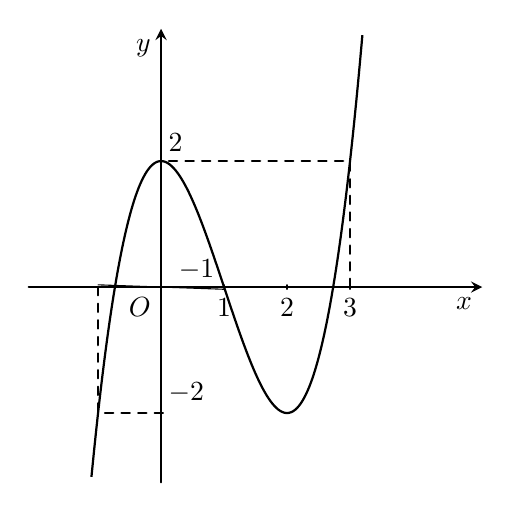
\begin{tikzpicture}[line join=round, line cap=round,>=stealth,thick,scale=.8]
		\tikzset{label style/.style={font=\footnotesize}}
		\draw[->] (-2.1,0)--(5.1,0) node[below left] {$x$};
		\draw[->] (0,-3.1)--(0,4.1) node[below left] {$y$};
		\draw (0,0) node [below left] {$O$};
		\foreach \x in {1,2,3}
		\draw[thin] (\x,1pt)--(\x,-1pt) node [below] {$\x$};
		\draw[thin](-1,1pt)--(1,-1pt)node[above left]{$-1$};
		\foreach \y in {-2,2}
		\draw[thin] (1pt,\y)--(-1pt,\y) node [above right] {$\y$};
		\begin{scope}
		\clip (-2,-3) rectangle (5,4);
		\draw[samples=200,domain=-2:4,smooth,variable=\x] plot (\x,{(\x)^3-3*(\x)^2+2});
		\end{scope}
		\draw[dashed] (-1,0)--(-1,-2)--(0,-2);
		\draw[dashed] (3,0)--(3,2)--(0,2);
		\end{tikzpicture}
	}
	\loigiai{
		\immini
		{
			Ta có $g'(x)=f'(x-m)-(x-m-1)$.\\
			$g(x)$ đồng biến trên $(5;6)\\ \Leftrightarrow g'(x)\ge 0\,\forall x\in (5;6)\\ \Leftrightarrow f'(x-m)\ge x-m-1\,\forall x\in (5;6)$.\\
			Đặt $t=x-m$, ta có  $f'(t)\ge t-1$.\\
			Dựa vào đồ thị ta có 
		}
		{
			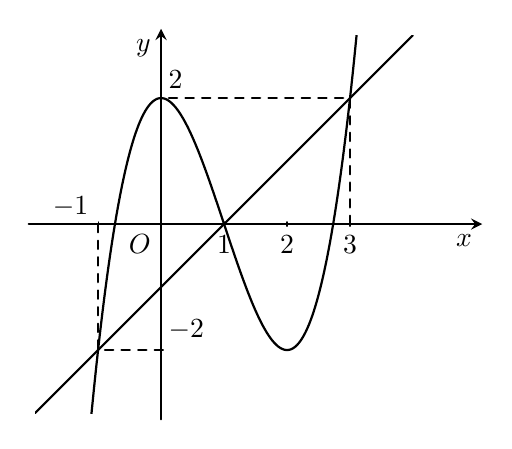
\begin{tikzpicture}[line join=round, line cap=round,>=stealth,thick,scale=.8]
			\tikzset{label style/.style={font=\footnotesize}}
			\draw[->] (-2.1,0)--(5.1,0) node[below left] {$x$};
			\draw[->] (0,-3.1)--(0,3.1) node[below left] {$y$};
			\draw (0,0) node [below left] {$O$};
			\foreach \x in {1,2,3}
			\draw[thin] (\x,1pt)--(\x,-1pt) node [below] {$\x$};
			\draw[thin](-1,1pt)--(-1,-1pt)node[above left]{$-1$};
			\foreach \y in {-2,2}
			\draw[thin] (1pt,\y)--(-1pt,\y) node [above right] {$\y$};
			\begin{scope}
			\clip (-2,-3) rectangle (5,3);
			\draw[samples=200,domain=-2:4,smooth,variable=\x] plot (\x,{(\x)^3-3*(\x)^2+2});
			\draw[samples=200,domain=-2:4,smooth,variable=\x] plot (\x,{(\x)-1});
			\end{scope}
			\draw[dashed] (-1,0)--(-1,-2)--(0,-2);
			\draw[dashed] (3,0)--(3,2)--(0,2);
			\end{tikzpicture}
		}
		\noindent
		\begin{eqnarray*}
			f'(t)\ge t-1&\Leftrightarrow &\hoac{&-1\le t\le 1\\&t\ge 3}\Leftrightarrow \hoac{&-1\le x-m\le 1\\&x-m\ge 3}\Leftrightarrow \hoac{&\heva{&m\ge x-1\\&m\le x+1}\\&m\le x-3}\\&\Leftrightarrow &\hoac{&\heva{&m\ge 6-1\\&m\le 5+1}\\&m\le 5-3}\Leftrightarrow\hoac{&5\le m\le 6\\&m\le 2.}
		\end{eqnarray*}
		Mà $m\in\mathbb{Z}^+$ nên $m\in\left \{1;2;5;6\right\} $.\\
		Tổng của các phần tử là $1+2+5+6=14$.
	}
\end{ex}


\Closesolutionfile{ans}
\begin{indapan}{10}
	{ans/ans-2-GHK1-33-NguyenTrai-QuangNam-21}
\end{indapan}